\documentclass[../main.tex]{subfiles}
\begin{document}

\chapter{Lecture 15 - 04-05-2020}
 
 \section{Regret analysis of OGD}
 We introduce the \bred{Regret}.
 \\
 $$
 \frac{1}{m} \ \sum_{t=1}^{T} \ell_t(w_t) - \frac{1}{T} \ \sum_{t=1}^{T} \ell_t(u^*_t) 
 $$
$$
(x_1,y_1) ...(x_t,y_t) \qquad \ell_t(w) = \left( w^T \, x_t - y_t\right)^2
$$
we build a loss function for example with the square loss.
\\
The important thing is that $\ell_1 , \ell_2, ...$ is a sequence of \textbf{convex losses}.
\\\\
In general we define the regret in this way:
$$
 R_T(u) \ =  \ \sum_{t=1}^{T} \ell_t(w_t) -  \sum_{t=1}^{T} \ell_t(u_t) 
$$\\
The Gradiant descent is one of the simplest algorithm for minimising a convex function. We recall the iteration did by the algorithm:
$$
w_{t+1} \leftarrow w_t - \eta_t \nabla f(w_t) \qquad \eta_t > 0 \textbf{  learning rate} \quad \textit{f convex} 
$$
$$
f: \barra{R}^d \rightarrow \barra{R} \textit{ that's why use the gradiand instead of the derivative}
$$
Learning rate can depend on time and we approach the region of the function f where the region is 0. We keep on moving in the X axes in the direction where the function is decreasing.
\newpage
\subsection{Projected OGD}

2 parameters: $\eta > 0$ and $U > 0$
\\
Initialisation: $ w_1 = (0,...,0)$
\\
For $t = 1,2,...$

1) \blue{Gradiant step}: 
$$w'_{t+1} = w_t - \frac{\eta}{\sqrt[]{t}} \ \nabla \ell_t(w_t) \qquad (x_t, y_t) \rightsquigarrow \ell_t
$$
\begin{figure}[h]
    \centering
    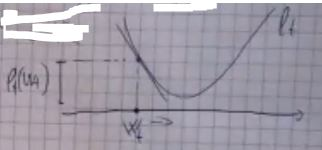
\includegraphics[width=0.3\linewidth]{../img/lez15-img1.JPG}
    \caption{}
    %\label{fig:}
\end{figure}\\

2) \blue{Projection step}: $$
w_{t+1} = arg \min_{w: \| w \| \leq U} \| w- w'_{t+1} \| $$ \textbf{Projection of $w'_{t+1}$ onto the ball of radius $U$}.
\begin{figure}[h]
    \centering
    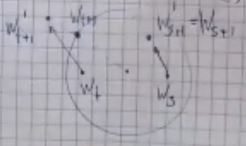
\includegraphics[width=0.3\linewidth]{../img/lez15-img2.JPG}
    \caption{}
    %\label{fig:}
\end{figure}\\
Now we define the Regret:
$$
U^*_T = arg \min_{U \in \barra{R}^d \ \|U \| \leq U} \frac{1}{T} \ \sum_{t=1}^{T} \ell_t(U)
$$
We are interested in bounding the regret $R_T\left(U^*_T\right) $
\\\\
I will Fix $\ell_1, ... \ell_t$ \qquad let $U= U^{\divideontimes}_T$ for $U$.
\\
Taylor's theorem for multivariate functions\\
Let's look a univariate first \quad $f: \barra{R} \rightarrow \barra{R}$ \textit{( has to be twice differentiable) }\qquad $w, u \in \barra{R}$
$$
f(u) = f(w) + f'(w) \, (u-w) + \frac{1}{2} \, f^"(x) \, (u-w)^2
$$
\\\\
For the multivariate case:
\\
$f: \barra{R}^d \rightarrow \barra{R} \quad$ twice differentiable \ $ \forall u, w \in \barra{R}^d$
$$
f(u) = f(w) + \nabla f(w)^T \, (u-w) + \frac{1}{2} \left(u-w\right)^T \nabla^2 f(\xi) \, (u-w)
$$
where $\xi$ is some point on the segment goining $u$ and $w$.
We have the Hessian matrix of $f$:
$$
\nabla^2 f(x)_{ij} \ = \ \frac{\partial^2 f(x)}{\partial x_i \, \partial x_j} \vert x=x_i
$$
If $f$ is convex then, $\nabla^2 f$ is positive and semidefinite.\\
$
\forall x \in \barra{R}^d \quad \forall z \in \barra{R}^d \qquad z^T \, \nabla^2 f(x) \, z \geq 0
$
\begin{figure}[h]
    \centering
    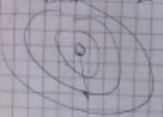
\includegraphics[width=0.3\linewidth]{../img/lez15-img3.JPG}
    \caption{}
    %\label{fig:}
\end{figure}\\
Now we can apply this results to our problem: in particular I rearrange the factors
$$
f(w) - f(u) \leq \nabla f(w)^T \, (w-u)
$$
This is Ok for $f$ convex and differentiable.
\\
I know that: $u-w^T\nabla^2 f(\xi) \, (u-w) \geq 0 $ because f is convex.
\\
$$
\ell_t(w_t) - \ell_t(u) \leq \nabla \ell_t (w_t)^T \, (w_t-u) \qquad \textbf{ Linear Regret}
$$\\
How do we proceed? \\
The first step of the algorithm is : $w'_{t+1} = w_t - \eta_t \nabla \ell_t(w_t) \qquad  \eta_t = \frac{\eta}{\sqrt[]{t}}$
$$
= - \frac{1}{\eta_t} \, (w'_{t+1} - w_t )^T \, (w_t-u) \ = \
 \frac{1}{\eta_t}\left( \frac{1}{2} \| w_t -u \|^2 - \frac{1}{2} \| w'_{t+1} - u \|^2 + \frac{1}{2} \|w_{t+1} - w_t \|^2 \right)  \ \leq
$$
$$
\leq \ 
 \frac{1}{\eta_t}\left( \frac{1}{2} \| w_t -u \|^2 - \frac{1}{2} \| w_{t+1} - u \|^2 + \frac{1}{2} \|w'_{t+1} - w_t \|^2 \right) 
$$
$w'$ disappear and add minus sign. I am saying that $\| w_{t+1} -u \| \leq \| w'_{t+1} - u\|$
\begin{figure}[h]
    \centering
    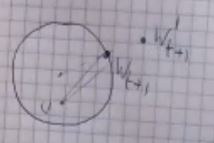
\includegraphics[width=0.3\linewidth]{../img/lez15-img4.JPG}
    \caption{}
    %\label{fig:}
\end{figure}\\
So is telling us that $w_{t+1}$ is closer to $u$ than $w'_{t+1}$
\\This holds since the ball is convex.
\\\\
Now we go back adding and subtracting $\pm \frac{1}{2 \, \eta_{t+1}} \| w_{t+1} -u \|^2$


$$
= \red{\frac{1}{2 \, \eta_t} \| w_t - u\|^2 - 
\frac{1}{2 \, \eta_{t+1}} \| w_{t+1} - u\|^2}
 -
 \blue{ $
 \frac{1}{2 \, \eta_{t}} \|w_{t+1}-u \|^2 
 +
 \frac{1}{2 \, \eta_{t+1}} \|w_{t+1}-u \|^2 $} 
+
\frac{1}{2 \, \eta_{t}} \|w_{t+1}- w_t \|^2 
$$
We group the 1,2 and 3,4 elements and sum them up. \\

$$
R_T(U) \ = \ \sum_{t=1}^{T} \left( \ell_t(w_t) - \ell_t(u) \right) \leq
$$
This is a \textbf{telescopic sum}:  $a_1-a_2+a_2-a_3+a_3-a_4+a_t -a_t+1$ and everything in the middle cancel out and remains first and last terms.
\\
$$
\leq  \frac{1}{2 \, \eta_t} \|w_1-u\|^2 - \frac{1}{\eta_{T+1}} \| w_{T+1} -u \| ^2 + \frac{1}{2} \sum_{t=1}^T \| w_{t+1} - u \|^2 \left( \frac{1}{\eta_{t+1}} - \frac{1}{\eta_t}\right) + \frac{1}{2} \sum_{t=1}^T \frac{\| w'_{t+1} -w_t \|^2}{\eta_t}
$$
where $w_1 = 0 $ \quad and  \quad $\| w_{t+1} - u \|^2 \leq 4 \, U^2$ \quad and \quad 
$
\| w'_{t+1} -w_t \|^2 = \eta_t^2 \| \nabla \ell_t (w_t) \|^2
$\\
We know that $\eta_t = \frac{\eta}{\sqrt[]{t}}$ \qquad so $\eta_1 = \frac{\eta}{\sqrt[]{1}} = \eta$
$$
R_T(U) \ \leq \ \frac{1}{2 \, \eta} U^2 
\red{
- \frac{1}{2 \, \eta_{T+1}} \|w_{T+1} - U \|^2 
}
+2 \, U^2 \, \sum_{t=1}^{T-1} \left(\frac{1}{\eta_t} - \frac{1}{\eta_t}\right)+
$$
$$ 
\red{
+ \frac{\| w_{T+1} -U \|^2}{2 \eta_{T+1}} - \frac{\| w_{T} -U \|^2}{\eta_T}  }
+ \frac{1}{2} \sum_{t=1}^T \eta_t \| \nabla \ell_t(w_t) \|^2 
$$
where \bred{red values} cancel out.
\\
I assume that square loss is bounded by some number $G^2$: $ \| \nabla \ell_t(w_t) \|^2 \ \leq \ G^2 $
\\
Also, it's a telescopic sum again and all middle terms cancel out.
\\
$$
\max_t \| \nabla_t(w_t) \|^2 \leq G
$$
$$
R_T(U) \leq \red{\frac{1}{2 \, \eta} U^2} + 2\, U^2 \left( \frac{1}{\eta_{T}} - \red{ \frac{1}{\eta_1} }\right) + \frac{G^2}{2} \, \eta \sum_{t=1}^T \frac{1}{\sqrt[]{t}} \qquad \eta_t = \frac{1}{\sqrt[]{t}}
$$
where \bred{red values} cancel out.
\\
Now how much is this sum $ \sum_{t=1}^T  \frac{1}{\sqrt[]{t}}$?
\\
It is bounder by the integral 
$
\leq \int_{1}^{T} \frac{dx}{\sqrt[]{x}} \leq 2 \, \sqrt[]{T}
$
$$
R_T(U) \ \leq \ \frac{2 \, U^2 \sqrt[]{T}}{\eta} + \eta \, G^2 \sqrt[]{T} \ = \ \left( \frac{2\, U^2}{\eta} + \eta \, G^2 \right) \, \sqrt[]{T} $$
$ \eta = \frac{U}{G} \sqrt[]{2}
$
\\
So finally:
$$
\frac{1}{T} \sum_{t=1}^T \ell_t(w_t) \leq \min_{\|U\| \leq U} \frac{1}{T} \sum_{t=1}^T \ell_t(u) + U \, G \ \sqrt[]{\frac{8}{T}}
$$
$$
R_T(U) = \frac{1}{T} \sum_{t=1}^T \left( \ell_t (w_t) - \ell_t(u) \right) \qquad \forall u : \|u\| \leq U : R_T(U) = O \left(\frac{1}{\sqrt[]{T}}\right)
$$
Basically my regret is gonna go to 0. 
\\\\
For $ERM in H$ where $| H| < \infty$, variance error vanishes at rate $\frac{1}{\sqrt[]{m}}$
\\\\
The bound $U \, G^2 \, \sqrt[]{\frac{8}{T}}$ on regret holds for any sequence $\ell_1, \ell_2, ...$ of convex and affordable losses, If $\ell_t(w) = \ell(w^T \, x_t, y_t)$ then the bound holds for any sequence of data points $(x_1,y_1), (x_2, y_2)..$
\\ 
This is not a statistical assumption but mathematical so stronger.
\end{document}